\documentclass[12pt]{article}
\oddsidemargin=0.0in
\evensidemargin=0.0in
\textwidth=6.5in
\topmargin=-0.55in
\textheight=9.3in
\usepackage{hyperref}
\usepackage{graphicx}

\begin{document}
\pagestyle{empty}
 
\begin{center}
{\LARGE {\bf Homework Four}}\\
\bigskip
{\Large {\bf Calculus I}}\\
\bigskip
{\Large {\bf College of the Atlantic}}\\
\bigskip
{ {\bf Due Friday, October 7, 2022}}\\ 
\end{center}
\medskip


\noindent There are two parts to this assignment.\\

\noindent {\bf Part 1: WeBWorK}.  Do Homework 04A, 04B, and 04C on
WeBWorK.  The WeBWorK page is here: 
\url{https://webwork.runestone.academy/webwork2/coa-feldman-es1024i-fall-2022/}.
I recommend doing the WeBWorK part of the homework first.  This will
enable you to benefit WeBWorK's instant feedback before you do part
two.\\ 


\noindent {\bf Part 2: Non-WeBWorK problems}.  Here are some
instructions for how to submit this part of the assignment.
\begin{itemize}
  \setlength{\itemsep}{0mm}
\item Do the problems by hand using pencil (or pen) and paper.
  There is no need to type this assignment.
%\item If you like working on a tablet, go for it. 
\item Make a pdf scan of your work using genius scan or some
  similar scanning app.  Please make the homework into a single
  pdf, not multiple pdfs.
\item Submit the assignment on google classroom.  Please don't
  email it to me.
  %(Between my two classes I will be receiving
  %around 60 assignments a week.  Keeping track of them all in email 
  %is challenging.)
\item If you want, you can do the non-WeBWorK problems in pairs and
  submit only one assignment for the two of you. \\
\end{itemize}

\noindent Here are some non-WeBWorK problems.


\begin{figure}[h]
\begin{center}
\vspace{1mm}
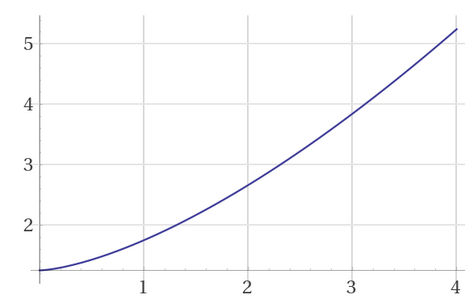
\includegraphics[width=3.0in]{graph_HW04_1.png}
\vspace{-1mm}
\caption{The position of a object (in meters) as a function of time
  (in seconds). }
\vspace{-5mm}
\label{fig:graph1}
\end{center}
\end{figure}
%\vspace{0mm}



\begin{enumerate}
\setlength{\itemsep}{8mm}


\item An object's position as a function of time is shown in
  Fig.~\ref{fig:graph1}. Use this graph to estimate:
  \begin{enumerate}
  \item The average speed between $t=1$ and $t=3$.
  \item The average speed between $t=1$ and $t=2$.
\end{enumerate}


\begin{figure}[h]
\begin{center}
\vspace{1mm}
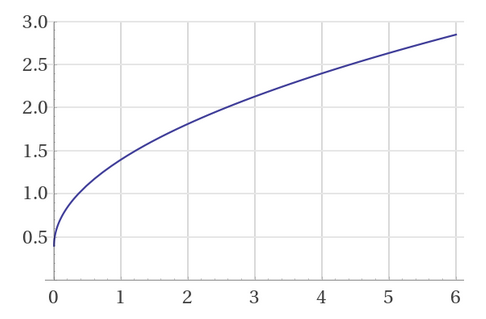
\includegraphics[width=3.0in]{graph_HW04_2.png}
\vspace{-2mm}
\caption{The position of a object (in meters) as a function of time
  (in seconds). }
\label{fig:graph2}
\vspace{-5mm}
\end{center}
\end{figure}
%\vspace{0mm}

\item An object's position as a function of time is shown in
  Fig.~\ref{fig:graph2}. On this graph draw:
  \begin{enumerate}
    \item A line whose slope is equal to the average speed of the
      object from $t=1$ to $t=4$.
    \item A line whose slope is equal to the instantaneous speed at
      $t=3$.
  \end{enumerate}



\item The position of a cat is given by $s(t) = t^3 + 2$, where $t$
  is measured in seconds and $s$ is measured in meters.
  \begin{enumerate}
  \item Find the average speed of the cat between time $2$ and time
    $2+h$ if: 
  \begin{enumerate}
  \item $h=0.1$
  \item $h=0.01$
  \item $h=0.100$
  \end{enumerate}
  \item What do you think is the instantaneous speed of the cat at
    time $t=2$?
  \end{enumerate}

\item Find the derivative of $f(x) = x^3 + 2$ at $x=2$ using algebra.
  That is, start with the definition of the derivative:
  \begin{equation}
    f^\prime(x) \, = \, \lim_{h\rightarrow 0} \frac{f(2+h) - f(x)}{h}
    \;.
    \end{equation}
Then use algebra to simplify the expression on the right. After a bit
of work, the $h$ downstairs will cancel and you'l be able to evaluate
the limit. Do not use any shortcuts you might have learned in other
classes, nor should you use a calculator to plug in values of $h$.

\item Repeat the above problem, but instead find the derivative of
  $g(x) = 1/x$ at $x=3$.  (This problem will involve a good bit more
  algebra than the last one.)

  
  
\end{enumerate}

\end{document}

  \setlength{\itemsep}{-1mm}
  \item Determine an equation for the linear function that generates
    the values in the table below.  

\begin{center}
\begin{tabular}{|| l | l ||}
\hline $x$ & $f(x)$ \\
\hline
5.2 & 27.8 \\
5.3 & 29.2 \\
5.4 & 30.6 \\
5.5 & 32.0 \\
5.6 & 33.4 \\
\hline
\end{tabular}
\end{center}





\end{document}
